\documentclass{beamer}
\usepackage{beamerthemeshadow}
\usepackage{graphicx}
\usepackage{color}
\usepackage[utf8]{inputenc}
\usepackage{hyperref}
\usepackage[english,serbian]{babel}
\usepackage[flushleft]{threeparttable}
\definecolor{beamer@darkblue}{rgb}{228, 0, 0}
\setbeamercolor{structure}{fg=beamer@darkblue}

\def\d{{\fontencoding{T1}\selectfont\dj}}
\def\D{{\fontencoding{T1}\selectfont\DJ}}

\title{Tehničko i naučno pisanje}
\subtitle{-- Nanotehnologija i primene --}
\author{Petar Đerić, Ivan Tešović, Luka Mijailović i Uroš Cvetković}
\institute{Matematički fakultet\\Univerzitet u Beogradu}
\date{
\footnotesize{26. decembar 2022.}
}

\begin{document}
\begin{frame}
\thispagestyle{empty}
\titlepage
\end{frame}

\addtocounter{framenumber}{-1}

\begin{frame}{Literatura}
\begin{itemize}
\item Vladimir Đoković, Nanotehnologije
\item MDPI, Nanomaterials
\item National Nanotechnology Initiative, Applications of Nanotechnology
\item Nanotechnology Advance Enables Tinier Transistors With Extraordinary Performance
\item How Do Nanomaterials Help Push the Boundaries in the Automotive Industry


\end{itemize}
\end{frame}

\begin{frame}
\frametitle{Pregled}
\tableofcontents[hidesubsections]
\end{frame}

\section{Uvod}

\begin{frame}{Uvod}
\begin{itemize}
\item Nano ($10^{-9}$) \\
\item Nano čestice i nano - lestvica
\item Norio Taniguči (Univerzitet u Tokiju, 1974. godine)

\item Da li je nanotehnologija nauka ili tehnologoja?
\item Progres u nanotehnologiji (preciznost, složenost, isplativost)
\item Tipični proizvodi nanotehnologije (nanočestice, fibre i filmovi)
\item Nano - roboti i self - healing materijali
\end{itemize}

\end{frame}

\section{Nanomaterijali}
\begin{frame}{Nanomaterijali}

\begin{itemize}
\item \textbf{Nanomaterijali} - objekti kojima je bar jedna dimenzija između 1 i 1000 nm
\begin{itemize}
\item \textbf{Nanocevi}
\item \textbf{Grafen}
\item \textbf{Fuleren}
\item \textbf{Kvantne tačke}
\item \textbf{Nanoljuske}
\end{itemize}
\end{itemize}

\begin{figure}[H]
\begin{center}
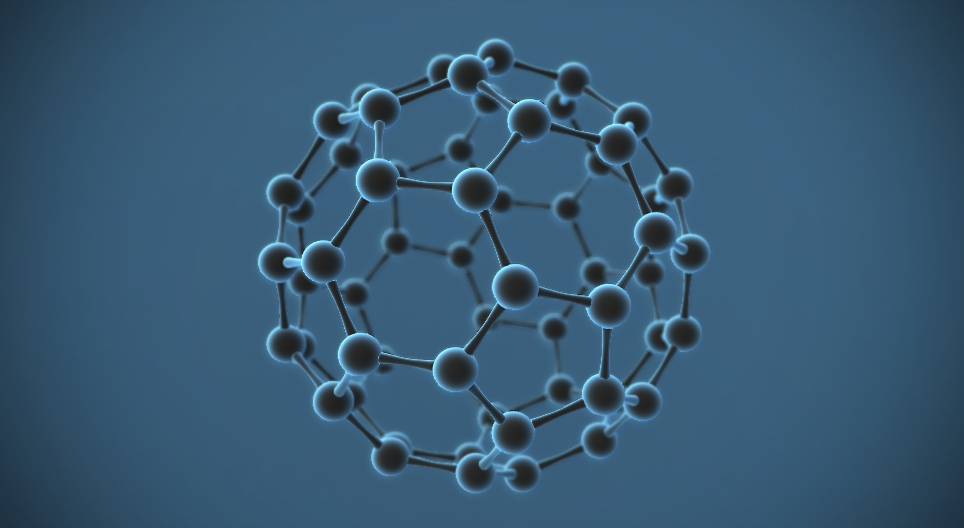
\includegraphics[scale=0.12]{slika 3.jpg}
\end{center}
\caption{Struktura fulerena}
\label{fig:slika_1}

\end{figure}
\end{frame}

\section{Primene nanotehnologije}
\begin{frame}{Primene nanotehnologije}
\begin{itemize}
\item \textbf{Nanotehnologija} ima široku primenu:
\begin{itemize}
\item IT industrija
\item Automobilska industrija
\item Elektronika
\item Medicinska industrija
\item Kvantna mehanika
\item Robotika
\end{itemize}
\end{itemize}

Pošto su primene nanotehnologije velike, mi ćemo vam predstaviti primenu u \textbf{IT
industriji} i u \textbf{automobilskoj industriji}.

\end{frame}
\begin{frame}{Primena u IT industriji}
\begin{itemize}
\item Revolucija i napredak
\item \textbf{Tranzistori}
\begin{itemize}
\item Stari - od 130 do 250 nanometara
\item Intel - 14 nanometara
\item IBM - 7 nanometara

\end{itemize}
\end{itemize}

2021. godine IBM pravi revolucionarni tranzistor od 2 nanometra koristeći 'nanolistove'

\end{frame}
\section{Primena nanotehnologije u automobilskoj industriji}
\begin{frame}{Primena nanotehnologije u automobilskoj industriji}
\begin{center}
\scalebox{0.65}{%
\begin{tabular}{|c|c|}
\hline
\textbf{Deo automobila} & \textbf{Nanomaterijal koji se koristi}\\
\hline
Spoljašnjost & nano-lak \\
Karoserija & nano-čelik \\
Unutrašnjost & nano-filter \\
Šasija i gume & crni ugljenik \\
\hline
\end{tabular}
}
\begin{itemize}
\item Primena nanotehnologije u proizvodnji karoserije automobila
\begin{itemize}
\item Nano-lak

\end{itemize}
\item Polimerska stakla
\end{itemize}
\end{center}
\end{frame}

\section{Zaključak}
\begin{frame}{Zaključak}
\begin{itemize}
\item Po očekivanjima mnogih nanotehnologija će obeležiti 21. vek i biće u stalnom
razvoju. Ova tehnologija razvija se u poslednjim decenijama neverovatnom brzinom, ali još uvek
je u ranoj fazi komercijalizacije.
\item Svakog dana se pojavljuje neka nova ideja o upotrebi nanotehnologije i veoma je
zanimljivo pratiti šta univerziteti, velike IT kompanije, medicinski i hemijski instituti imaju da
podele sa javnošću. Baš zbog toga mnogi kažu da je nanotehnologija sledeća \textbf{tehnološka
revolucija}.
\end{itemize}
\end{frame}

\end{document}